\chapter{Описание практической части}
\label{cha:ch_4}

При подготовке к созданию итоговой модели в первую очередь создавались симуляции (искуственные 
данные, похожие по статистическим распределениям на настоящие, но по своей структуре более простые). \\

После этого на созданных симуляциями данных тренировались первые образцы нейросетевых моделей. 

\begin{figure}
	\begin{minipage}[h]{0.32\linewidth}
		\center{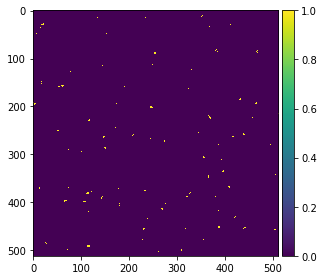
\includegraphics[width=\linewidth]{sym0}\\a)}
	\end{minipage}
	\begin{minipage}[h]{0.32\linewidth}
		\center{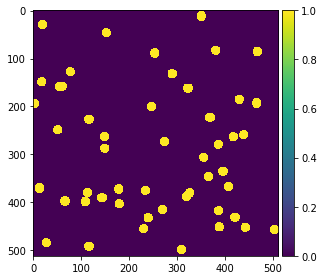
\includegraphics[width=\linewidth]{sym1}\\b)}
	\end{minipage}
	\begin{minipage}[h]{0.32\linewidth}
		\center{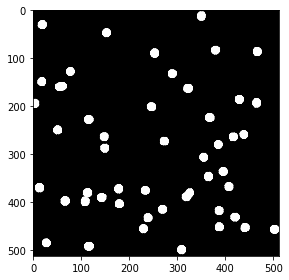
\includegraphics[width=0.9\linewidth]{sym2}\\c)}
	\end{minipage}

	\caption{a) Данные объектов из симуляций; b) Данные источников из симуляций; 
		c) Результат работы нейросети;}
\end{figure}

Выше приведен пример работы симуляции а также пример сегментированного изображения. Итоговая точность 
сегментации составляет 0.9978 для симулированных данных.\\

Далее, начинается обработка настоящих данных. Нужно загрузить и обработать каталог скоплений Planck, 
который будет разделен на два подкаталога: 
\begin{enumerate}
	\item planck\_z (скопления с измеренным красным сдвигом)
	\item planck\_no\_z (скопления без информации о красном сдвиге)
\end{enumerate}

После того, как были получены данные по скоплениям, можно начать загрузку и обработку данных из 
обзоров PS1. В каждом пикселе из разбиения с $n_{side}=2$ генеруется определенное количество патчей. 
Центры патчей выбираются случайным образом как пиксели из разбиения $n_{side}=11$. Размер каждого 
патча задан как 64 x 64, и так как пиксели HEALPix могут иметь протяжённую структуру, итоговый 
радиус патча вычислялся как расстояние от центра патча до дальнего угла для патча размером 66 x 66. 
В итоге радиус оказался равен $\approx 1.45^{\circ}$. \\

\begin{figure}[h]
	\begin{minipage}[h]{0.44\linewidth}
		\center{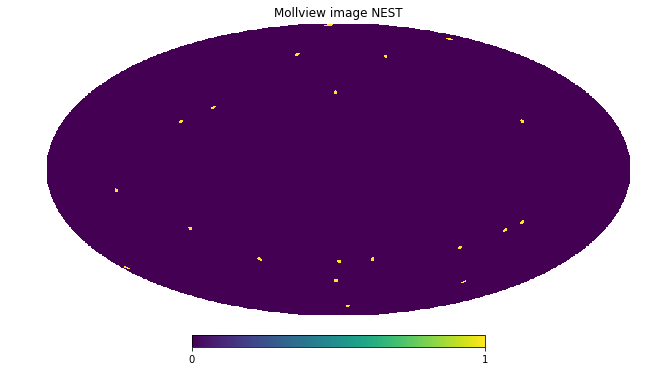
\includegraphics[width=\linewidth]{patch0}\\a)}
	\end{minipage}
	\begin{minipage}[h]{0.44\linewidth}
		\center{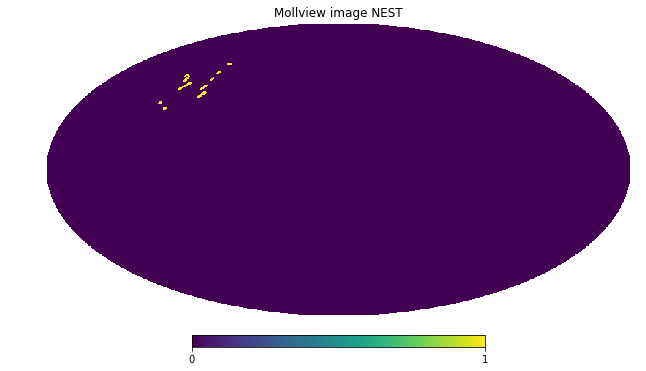
\includegraphics[width=\linewidth]{patch1}\\b)}
	\end{minipage}

	\caption{Сгенерированные центры патчей: a) Для всего неба; 
b) Для пикселя №6 из разбиения $n_{side}=2$;}
\end{figure}

Далее данные нужно преобразовать в формат двумерных матриц для загрузки в нейросеть. \\

\begin{figure}[h]
	\center{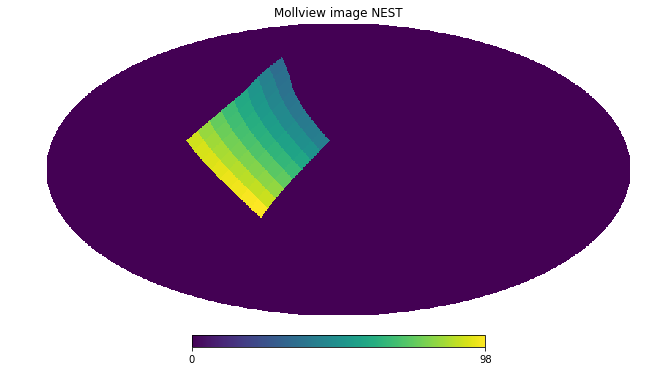
\includegraphics[width=0.8\linewidth]{pix2pic0}}
	\caption{Пример расположения двумерной матрицы на проекции неба для большего разбиения HEALPix}
\end{figure}
